\section {Sincronização via Ethernet com a BeagleBone Black}

\begin{frame}
\frametitle{Sincronização via Ethernet com a BBB }
\framesubtitle{Introdução}
\begin{itemize}
  \item Objetivo: avaliar o envio de \textit{triggers} de sincronismo via
  \textit{Ethernet}.
  \begin{itemize}
    \item Quantificar o \textit{jitter}, já que o \textit{delay} pode ser
    corrigido.
  \end{itemize}
  \item Propósito geral:
  \begin{itemize}
  \item \textit{BB1}: prepapar os
  pacotes \textit{UDP} contendo \textit{triggers} e enviá-los.
  
  \item \textit{BB2}: espera pacotes \textit{UDP}. Quando recebe, atualiza seu
  contador e seus pinos de saída.
  \end{itemize}
  \item 2 implementações realizadas: 
  \begin{itemize}
    \item \textit{Linux Kernel Modules}.
    \item PRU - \textit{Programmable Real-time Unit}.
  \end{itemize}
\end{itemize}
\end{frame}

\begin{frame}
\frametitle{Sincronização via Ethernet com a BBB }
\framesubtitle{Introdução}
\begin{itemize}
  \item Implementação dos \textit{Kernel Modules}:
\end{itemize}

\vspace{-12pt}

\begin{columns}

\begin{column}{.33\textwidth}

\begin{figure}[h!]
	
  \centering
  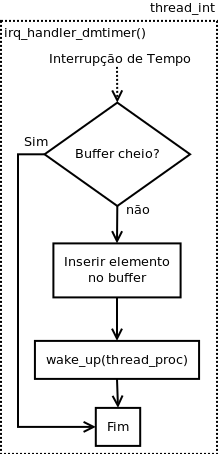
\includegraphics[scale=0.260]{image/thread_int}
  \caption{\centering BB1: \textit{thread} que é interrompida pelo
  \textit{timer}.}
  \label{fig:thread_int}
\end{figure}
\end{column}
		  
\begin{column}{.33\textwidth}

\begin{figure}[h!]
		  \centering
		  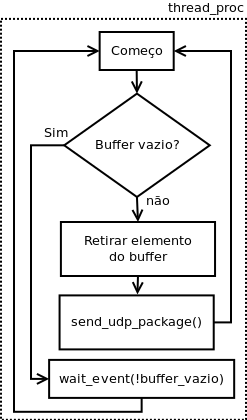
\includegraphics[scale=0.260]{image/thread_proc}
		  \caption{\centering BB1: \textit{thread} que envia pacotes à
		  rede.}
		  \label{fig:thread_proc} 
\end{figure}
\end{column}

\begin{column}{.33\textwidth}

\begin{figure}[h!]
			\centering
			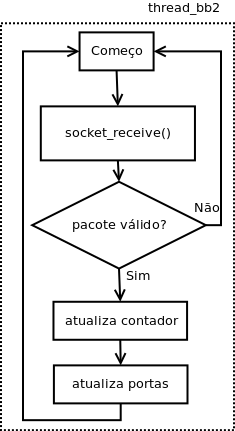
\includegraphics[scale=0.260]{image/thread_bb2}
			\caption {\centering \textit{thread} do \textit{kernel module}
			em
			\texttt{BB2}.}
			\label{fig:thread_bb2}
\end{figure}
\end{column}

\end{columns}
\end{frame}

\begin{frame}
\frametitle{Sincronização via Ethernet com a BBB }
\framesubtitle{Resultados}


\begin{columns}

\begin{column}{.5\textwidth}

\begin{figure}[h!]
\centering
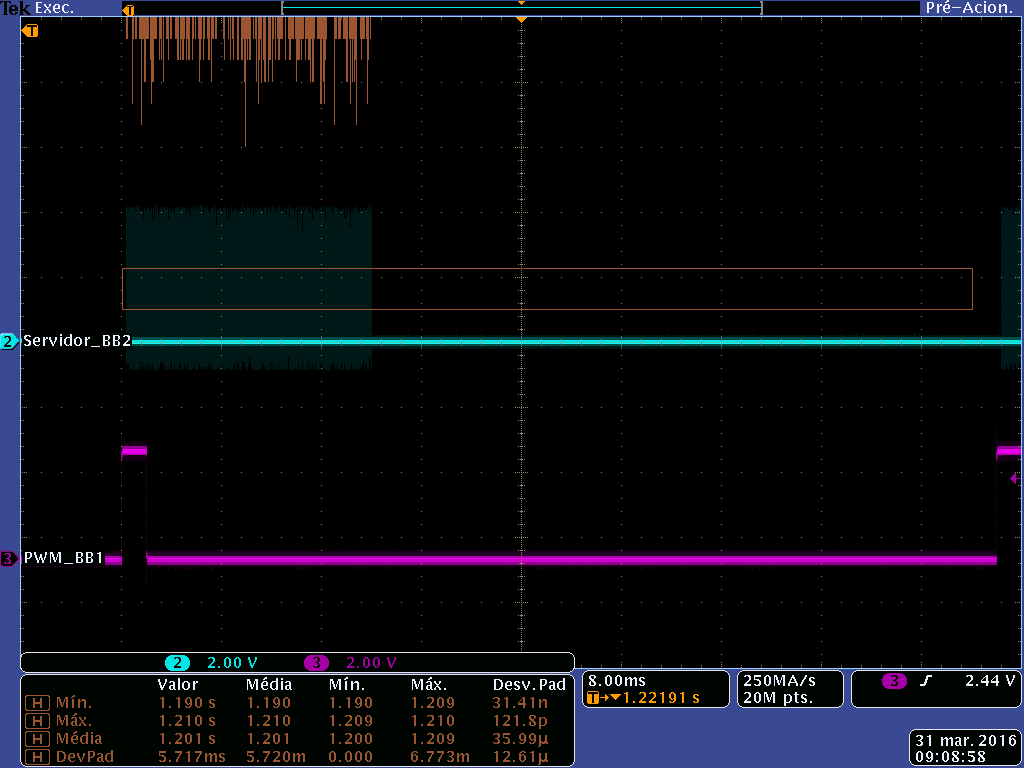
\includegraphics[width=\textwidth]{image/tek_com_threads}
\caption {\centering Captura de tela para a implementação com
\textit{kernel modules}.}
\label{fig:osciloscopio_thread}
\end{figure}
\end{column}%
\begin{column}{.5\textwidth}

\begin{figure}[h!]
\centering
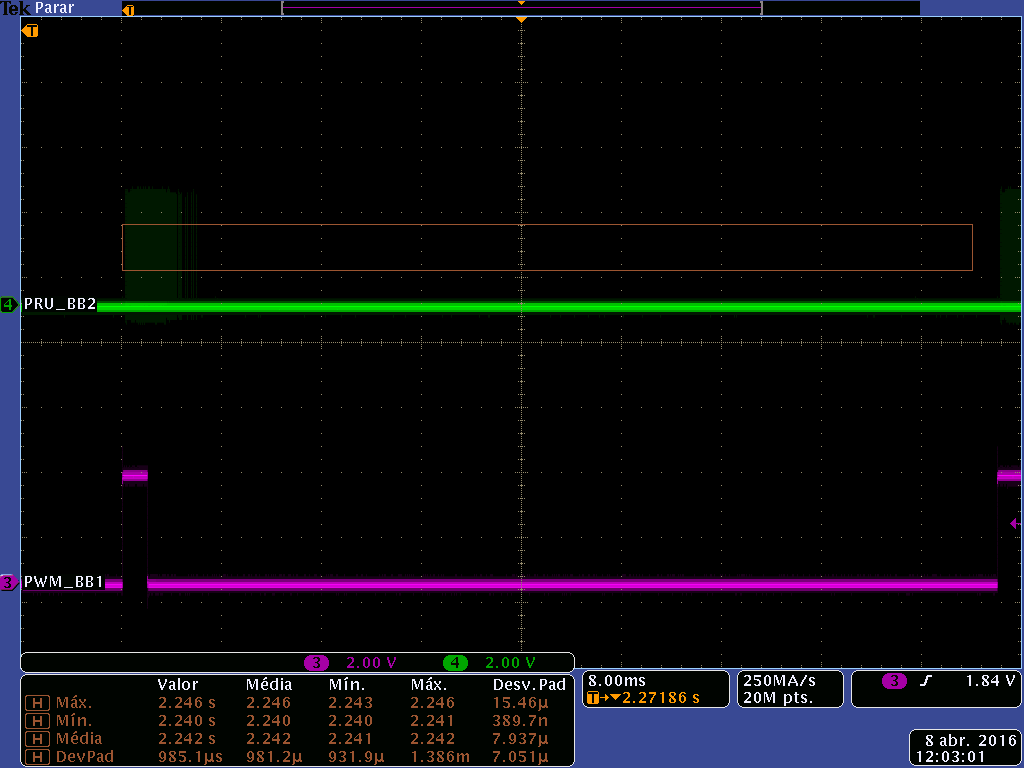
\includegraphics[width=\textwidth]{image/tek_pru}
\caption {\centering Captura de tela do osciloscópio para implementação com
PRU.}
\label{fig:pru_osciloscopio_thread}
\end{figure}
\end{column}

\end{columns}
\end{frame}